% !TeX root = ../../main.tex
% Add the above to each chapter to make compiling the PDF easier in some editors.

\section{Image Selection}\label{ord:ch4:sec4}

As the importance of a suitable dataset is already highlighted, this Section focuses on the composition of the benchmark dataset.
It was a conscious decision to select images from different domains and with different attributes.
Both, diverse domains and attributes, are fundamental to evaluate the generalization capability of the methods.
The selection of images for the dataset was done manually.
Thereby, images from various datasets are included: sPASCAL \gls{voc} \cite{Eve20-PascalVOC}, COCO \cite{Lin14-Coco}, DAVIS \cite{Per16-DAVIS}, CityScapes \cite{Cor16-Cityscapes}, \gls{d2s} \cite{Paddo18-D2S}, \gls{mad} \cite{Bergmann19-MAD}, MVTec Screws \cite{UFN19-Screws}, and other unpublished datasets from the MVTec Software GmbH.
% Other unpublsished MVTec Datasets
%--- pill_bags
%--- MVTec segmentation and counting dataset
%--- Single images: Cans, Cigarettes, Cereals
%--- MVTec closed packed & occluded object detection dataset (CPOD)
% Nachlabeln von Bildern
For some images from open source datasets the \gls{gt} was improved, in order to achieve a consistent goodness of the \gls{gt} for the benchmark dataset.

% Amount of images
The benchmark dataset contains 87 images with 133 annotations.
% Vergleichsweise klein
In the context of \gls{dl}, this evaluation datasets is comparatively small.
It was kept small on purpose, to enable users to label the majority of the images in a reasonable expenditure of time.
 
% es gibt kein 'perfektes' Dataset -> always depends on the porpuse of the model
It should be highlighted, that there is no \textit{ultimate} evaluation dataset, because the suitability of a dataset depends on the objective of the task.
Within the scope of this thesis, the main objective is to evaluate the generalization capabilities of interactive segmentation methods by real users.
The established dataset fulfills this evaluation purpose, as described in Chapter \ref{ord:ch5}.


\subsection{Domains}\label{ord:ch4:sec2:subsec1}

In order to ensure the variety of the benchmark dataset, each image was categorized into one of four domains:
%
\begin{itemize}
	\item \textbf{standard}, contains casual objects and scenes, that are common in daily life.
	The images mostly origin from \textit{general-use} datasets as PASCAL \gls{voc}, COCO, and DAVIS.
	\item \textbf{urban}, represents images of urban road scenes as in CityScapes.
	\item \textbf{industrial}, focuses on images from an industrial context, that are usually underrepresented in \textit{general-use} datasets.
	Images from \gls{d2s}, MVTec Screws, and other unpublished dataset are included.
	\item \textbf{anomaly}, contains images from the \gls{mad} dataset, which originally was used for anomaly detection.
	These images contain objects with defects such as cracks, contaminations, or holes.
\end{itemize}

An exemplary illustration of images from the different domains is presented in Figure \ref{fig:ch4:sec4:image_domains}, while multiple benchmark images are presented in \ref{fig:appendix_benchmark_domains}.

% Presentation of image domains.
\begin{figure} 
	\centering
	\begin{subfigure}[t]{0.45\textwidth}
		\centering
		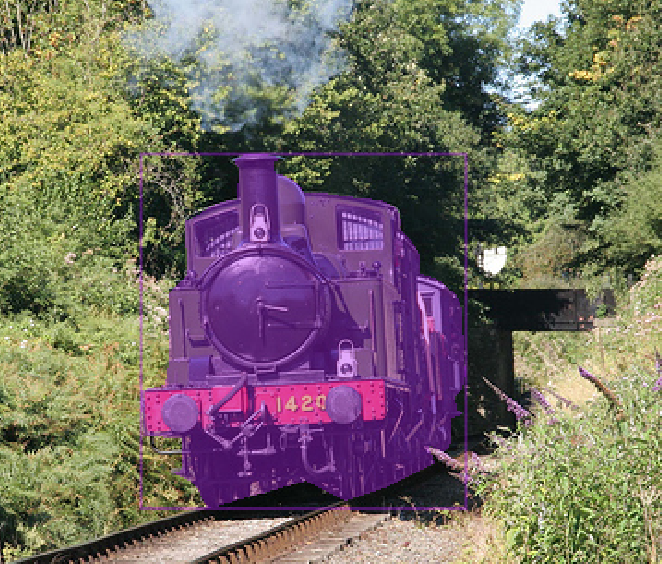
\includegraphics[width=\textwidth]{figures/chap44_standard.png}
		\caption{
			Example image from domain $ standard $.
		} \label{fig:ch4:sec4:domain_standard2}
	\end{subfigure}
	\hfill	
	\begin{subfigure}[t]{0.45\textwidth}
		\centering
		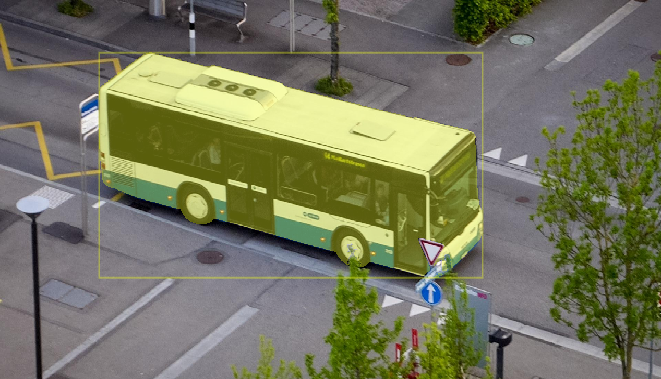
\includegraphics[width=\textwidth]{figures/chap44_urban.png}
		\caption{
			Example image from domain $ urban $.
		} \label{fig:ch4:sec4:domain_industrial}
	\end{subfigure}
	\\
	\begin{subfigure}[t]{0.45\textwidth}
		\centering
		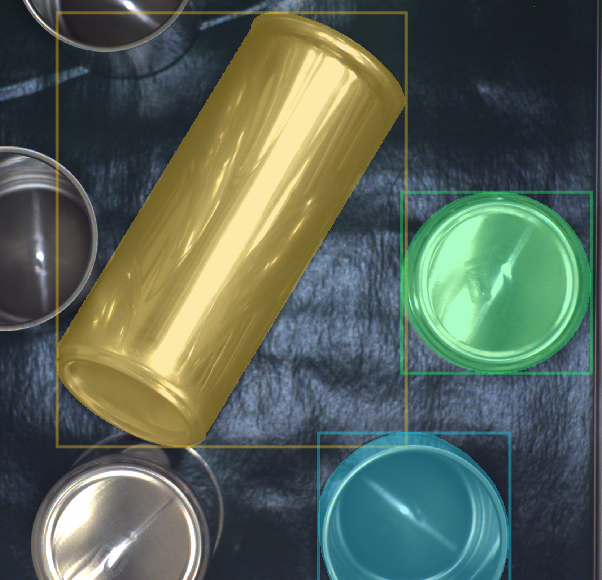
\includegraphics[width=\textwidth]{figures/chap44_industrial1.png}
		\caption{
			Example image from domain $ industrial $.
		} \label{fig:ch4:sec4:domain_urban}
	\end{subfigure}
	\hfill
	\begin{subfigure}[t]{0.45\textwidth}
		\centering
		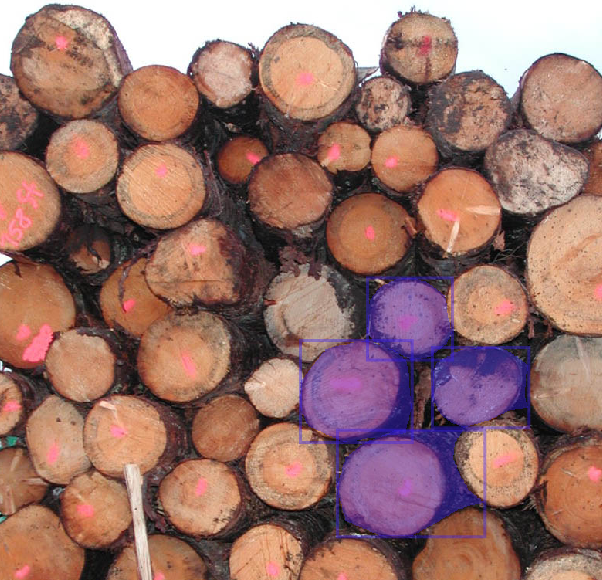
\includegraphics[width=\textwidth]{figures/chap44_industrial2.png}
		\caption{
			Example image from domain $ industrial $.
		} \label{fig:ch4:sec4:domain_standard}
	\end{subfigure}	
	\\
	\begin{subfigure}[t]{0.45\textwidth}
		\centering
		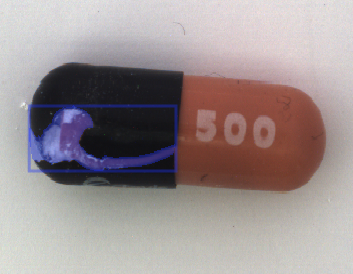
\includegraphics[width=\textwidth]{figures/chap44_anomaly1.png}
		\caption{
			Example image from domain $ anomaly $.
		} \label{fig:ch4:sec4:domain_anomaly1}
	\end{subfigure}
	\hfill
	\begin{subfigure}[t]{0.45\textwidth}
		\centering
		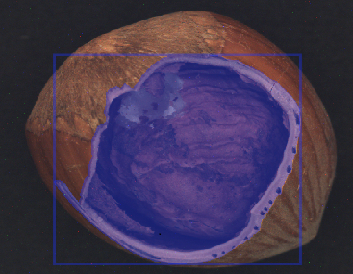
\includegraphics[width=\textwidth]{figures/chap44_anomaly2.png}
		\caption{
			Example image from domain $ anomaly $.
		} \label{fig:ch4:sec4:domain_anomaly2}
	\end{subfigure}	
	\caption[Illustration of benchmark images]{
		Presentation of benchmark images from the domain $ standard $, $ urban $, $ industrial $, and $ anomaly $, to show the diversity between the domains.
	} \label{fig:ch4:sec4:image_domains}
\end{figure}

% State of the art
\begin{table}[h!]
	\centering
	\begin{tabular}{l|c c c c}
		Domain				& $ standard $ & $ urban $ & $ industrial $ & $ anomaly $ \\
		\hline
		Number of images 	& 21 & 12 & 31 & 23 \\
		Number of object 	& 24 & 15 & 73 & 23 \\
	\end{tabular}
	\caption[Overview of image domains]{
		Distribution of the benchmark images over the four image domains.
		An image may contain multiple objects to annotate, that belong to the same image domain.
	} \label{tab:ch4:domains_overview}
\end{table}



\subsection{Attributes}\label{ord:ch4:sec2:subsec2}

The attributes of the benchmark images and objects also impact the segmentation and evaluation.
In order to create a balanced benchmark dataset, the selection of each image is not only based on the image domains, but also based on these attributes.
In general, the image attributes also could be used to further evaluate the generalization capabilities in detail, but this in not realized within the scope of this thesis.
The following attribute categories have been established and assigned for each image.

\begin{itemize}
	\item \textbf{Illumination}, states if an image is underexposed, overexposed, or normal.
	\item \textbf{Color channel}, differentiates between \gls{rgb} and gray scale images.
	\item \textbf{Contrast}, states if the contrast in the image is high or low.
	\item \textbf{Shapes}, describes the shape of the object as convex, uneven, or if it contains holes.
	\item \textbf{Overlap}, states if multiple objects are touching, overlapping, or there is no contact at all.
	\item \textbf{Number of objects}, gives a simplified idea about the amount of objects in the image (single, few, or many).
	\item \textbf{Error type}, describes the type of error for images of the domain \textit{anomaly}.
	The error types categories are \textit{holes}, \textit{cracks}, \textit{contamination}, or \textit{none} as default.
	\item \textbf{Reflection}, binary describes if the objects are reflecting.
	\item \textbf{Background texture}, describes the background of the image as plain, textured, or cluttered.
	\item \textbf{Foreground texture}, describes the foreground of the image as plain, textured, or cluttered.
\end{itemize}